\documentclass[10pt]{beamer}
\usetheme{Warsaw}
\usecolortheme{beaver}

\usepackage{amssymb, amsmath, amsfonts}
\usepackage{moreverb}
\usepackage{graphicx}
\usepackage{enumerate}
\usepackage{graphics}
\usepackage{color}
\usepackage{array}
\usepackage{float}
\usepackage{hyperref}
\usepackage{textcomp}
\usepackage{alltt}
\usepackage{mathtools}
\usepackage{tikz}
\usetikzlibrary{arrows}
\usepackage{bigints}

\newcommand{\suchthat}{\, \mid \,}
\renewcommand{\theenumi}{\alph{enumi}}
\newcommand\Wider[2][3em]{%
\makebox[\linewidth][c]{%
  \begin{minipage}{\dimexpr\textwidth+#1\relax}
  \raggedright#2
  \end{minipage}%
  }%
}
\setcounter{section}{-1}
%\setlength{\jot}{30pt}

\title{The Ecological Effects of Trait Variation in a $u$-Predator, $v$-Prey System}
\author{Sam Fleischer, Pablo Chavarria}
\date{March 14, 2015}

\begin{document}

\begin{frame}
	\titlepage
\end{frame}

\section{Introduction}
\begin{frame}
	\frametitle{}
	{\bf Advisors}
	\begin{itemize}
		\item Dr. Jing Li \\
		Assistant Professor, CSU Northridge \\
		Department of Mathematics
		\item Dr. Casey terHorst \\
		Assistant Professor, CSU Northridge \\
		Biology Department
	\end{itemize}
	{\bf Funding}
	\begin{itemize}
		\item National Science Foundation \\
		Pacific Math Alliance \\
		Preparing Undergraduates through Mentoring towards PhDs (PUMP)
	\end{itemize}
\end{frame}

\section{Motivation}
\begin{frame}
	\frametitle{}
	{\bf Observations}
	\begin{itemize}
		\item Predator/Prey interactions are prevalent in nature
		\begin{itemize}
			\item Crab vs. gastropod
			\item Protist vs. bacteria
		\end{itemize}
		\item There is trait variation within species
		\begin{itemize}
			\item Thickness of plant cuticula
			\item Strength of gastropod shell
		\end{itemize}
		\item Incorporating trait variation provides richer dynamics than classical Lotka-Volterra models
	\end{itemize}
\end{frame}

\section{Model Formulation}
\subsection{Lotka-Volterra}
\begin{frame}
	\frametitle{Classical Lotka-Volterra Model}
	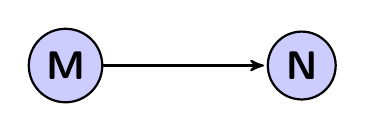
\begin{tikzpicture}[->,>=stealth',shorten >=1pt,auto,node distance=3cm,
		thick,main node/.style={circle,fill=blue!20,draw,font=\sffamily\Large\bfseries}]

		\node[main node] (1) {M};
		\node[main node] (2) [right of=1] {N};

		\path[every node/.style={font=\sffamily\small}]
		(1) edge [right] node[left] {} (2);
	\end{tikzpicture}
	\begin{align*}
		\frac{dN}{dt} &= N(r - \alpha M)\\[.1cm]
		\frac{dM}{dt} &= M(e\alpha N - d)
	\end{align*}
	{\bf Variables}
	\begin{itemize}
		\item $N \equiv $ Prey Density
		\item $M \equiv $ Predator Density
	\end{itemize}
	{\bf Parameters}
	\begin{itemize}
		\item $\alpha \equiv $ Attack rate \uncover<2->{{\color{red}\ \ \ \ \ $\longleftarrow$ {\it No variation!}}}
		\item $r \equiv $ Prey birth rate
		\item $e \equiv $ Efficiency
		\item $d \equiv $ Predator death rate
	\end{itemize}
\end{frame}
\subsection{Schreiber, B\"urger, and Bolnick}
\begin{frame}
	\frametitle{Schreiber, B\"urger, and Bolnick's Extension}
	\begin{align*}
		a(m) = \alpha \exp\left[-\frac{(m - \theta)^2}{2\tau^2}\right]
	\end{align*}
	{\bf Variables}
	\begin{itemize}
		\item $N \equiv $ Prey Density
		\item $M \equiv $ Predator Density
		\item \uncover<2->{{\color{red} No Prey Character}}
		\item $m \equiv $ Predator Character (Trait Value)
	\end{itemize}
	{\bf Parameters}
	\begin{itemize}
		\item $\alpha \equiv $ Maximum attack rate
		\item $\theta \equiv $ Optimal trait value \uncover<2->{{\color{red}\ \ \ \ \ $\longleftarrow$ {\it No variation!}}}
		\item $\tau \equiv $ Specialization Constant
	\end{itemize}
\end{frame}
\subsection{Our Extension}
\begin{frame}
	\frametitle{Our Extension}
	\begin{align*}
		a(m, n) = \alpha \exp\left[-\frac{(m - n - \theta)^2}{2\tau^2}\right]
	\end{align*}
	{\bf Variables}
	\begin{itemize}
		\item $N \equiv $ Prey Density
		\item $M \equiv $ Predator Density
		\item $n \equiv $ Prey Character (Trait Value)
		\item $m \equiv $ Predator Character (Trait Value)
	\end{itemize}
	{\bf Parameters}
	\begin{itemize}
		\item $\alpha \equiv $ Maximum attack rate
		\item $\theta \equiv $ Optimal trait {\color{red}\it difference}
		\item $\tau \equiv $ Specialization Constant
	\end{itemize}
\end{frame}
\begin{frame}
	\frametitle{}
	{\bf Distribution Assumptions}
	\begin{itemize}
		\item Trait values are {\bf normally distributed} over the populations
	\end{itemize}
	\begin{align*}
		p(n, \overline{n}) &= \frac{1}{\sqrt{2\pi\beta^2}}\exp\left[{-\frac{(n - \overline{n})^2}{2\beta^2}}\right] \\
		p(m, \overline{m}) &= \frac{1}{\sqrt{2\pi\sigma^2}}\exp\left[{-\frac{(m - \overline{m})^2}{2\sigma^2}}\right]
	\end{align*}
	{\bf Variables}
	\begin{itemize}
		\item $N \equiv $ Prey Density
		\item $\overline{n} \equiv $ Mean Prey Character
		\item $M \equiv $ Predator Density
		\item $\overline{m} \equiv $ Mean Predator Character
	\end{itemize}
	{\bf Parameters}
	\begin{itemize}
		\item $\beta^2 \equiv $ Prey Trait Variance
		\item $\sigma^2 \equiv $ Predator Trait Variance
	\end{itemize}
\end{frame}
\begin{frame}
	\frametitle{}
	{\bf Average Attack Rate}
	\begin{align*}
		\overline{a}(\overline{m}, \overline{n}) &= \int_{-\infty}^{\infty}\int_{\-\infty}^{\infty} a_{}(m, n) \cdot p(m, \overline{m}) \cdot p(n, \overline{n}) dm dn \\
		&= \frac{\alpha\tau}{\sqrt{\sigma^2 + \beta^2 + \tau^2}}\exp\left[{-\frac{(\overline{m} - \overline{n} - \theta)^2}{2(\sigma^2 + \beta^2 + \tau^2)}}\right]
	\end{align*}
	{\bf Variables}
	\begin{itemize}
		\item $N \equiv $ Prey Density
		\item $\overline{n} \equiv $ Mean Prey Character
		\item $M \equiv $ Predator Density
		\item $\overline{m} \equiv $ Mean Predator Character
	\end{itemize}
	{\bf Parameters}
	\begin{itemize}
		\item $\beta^2 \equiv $ Prey Trait Variance
		\item $\sigma^2 \equiv $ Predator Trait Variance
		\item $\alpha \equiv $ Maximum attack rate
		\item $\theta \equiv $ Optimal trait difference
		\item $\tau \equiv $ Specialization Constant
	\end{itemize}
\end{frame}
\begin{frame}
	\frametitle{}
	{\bf Fitness Assumptions}
	\begin{itemize}
		\item Prey experiences {\color{red}logistic growth} in absence of predator
		\item Predator experiences {\color{blue} exponential decay} in absence of prey
	\end{itemize}
	\begin{align*}
		Y(m, n, M, N) &= {\color{red}r\left(1 - \frac{N}{K}\right)} - Ma(m, n) \\[.1cm]
		W(m, n, N) &= eNa(m, n)\ {\color{blue} -\ d}
	\end{align*}
	{\bf Variables}
	\begin{itemize}
		\item $N \equiv $ Prey Density
		\item $n \equiv $ Prey Character
		\item $M \equiv $ Predator Density
		\item $m \equiv $ Predator Character
	\end{itemize}
	{\bf Parameters}
	\begin{itemize}
		\item $r \equiv $ Intrinsic Prey Growth Rate
		\item $K \equiv $ Prey Carrying Capacity
		\item $d \equiv $ Predator Death Rate
		\item $e \equiv $ Efficiency
	\end{itemize}
\end{frame}
\begin{frame}
	\frametitle{}
	{\bf Average Fitness}
	\begin{align*}
	\overline{Y}(\overline{m}, \overline{n}, M, N) &= \int_{-\infty}^{\infty}\int_{-\infty}^{\infty} Y(m, n, M, N) \cdot p(m, \overline{m}) \cdot p(n, \overline{n}) dm dn \\
	&= r\left(1 - \frac{N}{K}\right) - M\overline{a}(\overline{m}, \overline{n}) \\[.1cm]
	\overline{W}(\overline{m}, \overline{n}, N) &= \int_{-\infty}^{\infty}\int_{-\infty}^{\infty} W(m, n, N) \cdot p(m, \overline{m}) \cdot p(n, \overline{n}) dm dn \\
	&= eN\overline{a}(\overline{m}, \overline{n}) - d
	\end{align*}
	{\bf Variables}
	\begin{itemize}
		\item $N \equiv $ Prey Density
		\item $\overline{n} \equiv $ Mean Prey Character
		\item $M \equiv $ Predator Density
		\item $\overline{m} \equiv $ Mean Predator Character
	\end{itemize}
	{\bf Parameters}
	\begin{itemize}
		\item $r \equiv $ Intrinsic Prey Growth Rate
		\item $K \equiv $ Prey Carrying Capacity
		\item $d \equiv $ Predator Death Rate
		\item $e \equiv $ Efficiency
	\end{itemize}
\end{frame}
\begin{frame}
	\frametitle{}
	{\bf Ecological Components}
	\begin{align*}
		\frac{dN}{dt} &= N\cdot {\color{red}\overline{Y}(\overline{m}, \overline{n}, M, N)}= N{\color{red}\left[r\left(1 - \frac{N}{K}\right) - M\overline{a}(\overline{m}, \overline{n})\right]}\\[.1cm]
		\frac{dM}{dt} &= M\cdot {\color{blue}\overline{W}(\overline{m}, \overline{n}, N)}\ \ \ = M{\color{blue}\left[eN\overline{a}(\overline{m}, \overline{n}) - d\right]}
	\end{align*}
	{\bf Variables}
	\begin{itemize}
		\item $N \equiv $ Prey Density
		\item $\overline{n} \equiv $ Mean Prey Character
		\item $M \equiv $ Predator Density
		\item $\overline{m} \equiv $ Mean Predator Character
	\end{itemize}
	{\bf Parameters}
	\begin{itemize}
		\item $r \equiv $ Intrinsic Prey Growth Rate
		\item $K \equiv $ Prey Carrying Capacity
		\item $d \equiv $ Predator Death Rate
		\item $e \equiv $ Efficiency
	\end{itemize}
\end{frame}
\begin{frame}
	\frametitle{}
	{\bf Evolutionary Components}
	\begin{itemize}
		\item The evolution of the mean character is always {\color{red} in the direction which increases the mean fitness in the population}.
	\end{itemize}
	\begin{align*}
	\frac{d\overline{n}}{dt} &= \beta_G^2{\color{magenta}\frac{\partial \overline{Y}}{\partial \overline{n}}} = \beta_G^2{\color{magenta}\frac{M(\theta + \overline{n} - \overline{m})}{\sigma^2 + \beta^2 + \tau^2} \overline{a}(\overline{m}, \overline{n})}\\[.1cm]
	\frac{d\overline{m}}{dt} &= \sigma_G^2{\color{cyan}\frac{\partial \overline{W}}{\partial \overline{m}}} = \sigma_G^2{\color{cyan}\frac{eN(\theta + \overline{n} - \overline{m})}{\sigma^2 + \beta^2 + \tau^2} \overline{a}(\overline{m}, \overline{n})}\\
	\end{align*}
	{\bf Variables}
	\begin{itemize}
		\item $N \equiv $ Prey Density
		\item $\overline{n} \equiv $ Mean Prey Character
		\item $M \equiv $ Predator Density
		\item $\overline{m} \equiv $ Mean Predator Character
	\end{itemize}
	{\bf Parameters}
	\begin{itemize}
		\item $\beta_G^2 \equiv $ Prey genetic variance
		\item $\sigma_G^2 \equiv $ Predator genetic variance
	\end{itemize}
\end{frame}
\begin{frame}
	\frametitle{The Complete $1\times1$ Model \\ (One Predator Species, One Prey Species)}
	{\bf Ecological Components}
	\begin{align*}
	\frac{dN}{dt} &= N\cdot {\color{red}\overline{Y}(\overline{m}, \overline{n}, M, N)}\ \ =\ N{\color{red}\left[r\left(1 - \frac{N}{K}\right) - M\overline{a}(\overline{m}, \overline{n})\right]}\\[.1cm]
	\frac{dM}{dt} &= M\cdot {\color{blue}\overline{W}(\overline{m}, \overline{n}, N)}\ \ \ \ \ =\ M{\color{blue}\left[eN\overline{a}(\overline{m}, \overline{n}) - d\right]}
	\end{align*}
	{\bf Evolutionary Components}
	\begin{align*}
	\frac{d\overline{n}}{dt} &= \beta_G^2{\color{magenta}\frac{\partial \overline{Y}}{\partial \overline{n}}} = \beta_G^2{\color{magenta}\frac{M(\theta + \overline{n} - \overline{m})}{\sigma^2 + \beta^2 + \tau^2} \overline{a}(\overline{m}, \overline{n})}\\[.1cm]
	\frac{d\overline{m}}{dt} &= \sigma_G^2{\color{cyan}\frac{\partial \overline{W}}{\partial \overline{m}}} = \sigma_G^2{\color{cyan}\frac{eN(\theta + \overline{n} - \overline{m})}{\sigma^2 + \beta^2 + \tau^2} \overline{a}(\overline{m}, \overline{n})}
	\end{align*}
\end{frame}
\begin{frame}
	\frametitle{}
	{\bf Prey Fitness}
	\begin{align*}
		Y(m, n, M, N) &= r\left(1 - \frac{N}{K}\right) - Ma(m, n) \\
		\uncover<2->{&\downarrow} \\
		\uncover<2->{Y_j([m_i]_{i=1}^{u}, n_j, [M_i]_{i=1}^{u}, N_j) &= r_j\left(1 - \frac{N_j}{K_j}\right) - \sum\limits_{i = 1}^{u}M_ia_{ij}(m_i, n_j)}
	\end{align*}
	{\bf Predator Fitness}
	\begin{align*}
		W(m, n, N) &= eNa(m, n) - d \\
		\uncover<3->{&\downarrow} \\
		\uncover<3->{W_i(m_i, [n_j]_{j=1}^{v}, [N_j]_{j=1}^{v}) &= \sum\limits_{j = 1}^{v}\Big[e_{ij}N_ja_{ij}(m_i, n_j)\Big] - d_i}
	\end{align*}
	\uncover<2->{{\bf Notation}}
	\begin{align*}
		\uncover<2->{[x_i]_{i=1}^{u} = x_1, \dots, x_u}
	\end{align*}
\end{frame}
\begin{frame}
	\frametitle{}
	{\bf Average Fitness}
	\begin{align*}
		\overline{Y}_j([\overline{m}_i]_{i=1}^{u}, \overline{n}_j,\ &[M_i]_{i=1}^{u}, N_j) \\
		&= \int\limits_{\mathbb{R}^{u+1}} Y_j \cdot \prod\limits_{i=1}^{u}\Big[p_i(m_i, \overline{m_i})\Big] \cdot p(n, \overline{n}) \prod\limits_{i=1}^{u}\Big[dm_i\Big] dn_j\\
		&= r_j\left(1 - \frac{N_j}{K_j}\right) - \sum\limits_{i = 1}^{u}M_i\overline{a}_{ij}(\overline{m}_i, \overline{n}_j)
	\end{align*}
	\begin{align*}
		\overline{W}_i(\overline{m}_i, [\overline{n}_j]_{j=1}^{v}, [&N_j]_{j=1}^{v}) \\
		&= \int\limits_{\mathbb{R}^{u+1}} W_i \cdot p_i(m_i, \overline{m_i}) \cdot \prod\limits_{j=1}^{v}\Big[p(n_j, \overline{n}_j)\Big] dm_i \prod\limits_{j=1}^{v}\Big[dn_j\Big]\\
		&= \sum\limits_{j = 1}^{v}\Big[e_{ij}N_j\overline{a}_{ij}(\overline{m}_i, \overline{n}_j)\Big] - d_i
	\end{align*}
\end{frame}
\begin{frame}
	\frametitle{The Complete $u\times v$ Model \\ ($u$ Predator Species, $v$ Prey Species)}
	{\bf Ecological Components}
	\begin{align*}
		\frac{dN_j}{dt} &= N_j{\color{red}\overline{Y}_j} = N_j {\color{red}\left[r_j\left(1 - \frac{N_j}{K_j}\right) - \sum\limits_{i = 1}^{u}M_i\overline{a}_{ij}(\overline{m}_i, \overline{n}_j)\right]} \\[.1cm]
		\frac{dM_i}{dt} &= M_i{\color{blue}\overline{W}_i} = M_i {\color{blue}\left[\sum\limits_{j = 1}^{v}\Big[e_{ij}N_j\overline{a}_{ij}(\overline{m}_i, \overline{n}_j)\Big] - d_i\right]}
	\end{align*}
	{\bf Evolutionary Components}
	\begin{align*}
	\frac{d\overline{n}_j}{dt} &= \beta_{Gj}^2{\color{magenta}\frac{\partial \overline{Y}_j}{\partial \overline{n}_j}} = \beta_{Gj}^2{\color{magenta}\sum\limits_{i=1}^{u}\left[\frac{M_i(\theta_{ij} + \overline{n_j} - \overline{m_i})}{\sigma_i^2 + \beta_j^2 + \tau_{ij}^2} \overline{a}_{ij}(\overline{m_i}, \overline{n_j})\right]}\\[.1cm]
	\frac{d\overline{m}_i}{dt} &= \sigma_{Gi}^2{\color{cyan}\frac{\partial \overline{W}_i}{\partial \overline{m}_i}} = \sigma_{Gi}^2{\color{cyan}\sum\limits_{j=1}^{v}\left[\frac{e_{ij}N_j(\theta_{ij} + \overline{n_j} - \overline{m_i})}{\sigma_i^2 + \beta_j^2 + \tau_{ij}^2} \overline{a}_{ij}(\overline{m_i}, \overline{n_j})\right]}
	\end{align*}
\end{frame}

\section{Preliminary Results}
\subsection{$1 \times 1$}
\begin{frame}
	\frametitle{Equilibria - $1\times1$}
	\begin{align*}
		\begin{array}{ll}
			\dfrac{dN}{dt} = N\cdot \overline{Y}(\overline{m}, \overline{n}, M, N) &\ \ \ \ \ \ \dfrac{d\overline{n}}{dt} = \beta_G^2\dfrac{\partial \overline{Y}}{\partial \overline{n}} \\[.3cm]
			\dfrac{dM}{dt} = M\cdot \overline{W}(\overline{m}, \overline{n}, N) & \ \ \ \ \ \ \dfrac{d\overline{m}}{dt} = \sigma_G^2\dfrac{\partial \overline{W}}{\partial \overline{m}}
		\end{array}
	\end{align*}
	{\bf Extinction} \uncover<2->{$\boxed{\text{\it Unstable}}$}
	\begin{align*}
		(N^*, M^*, \overline{n}^*, \overline{m}^*) = (0, 0, \underline{\ \ }, \underline{\ \ })
	\end{align*}
	{\bf Exclusion} \uncover<3->{$\boxed{\text{\it Stable under certain conditions}}$}
	\begin{align*}
		(N^*, M^*, \overline{n}^*, \overline{m}^*) = (K, 0, \underline{\ \ }, \underline{\ \ })
	\end{align*}
	\uncover<4->{{\bf Necessary Conditions for Stable Exclusion:}}
	\begin{itemize}
		\item \uncover<4->{$d > e\overline{a}(\overline{m}^*, \overline{n}^*)K$}
		\item \uncover<4->{$(\overline{m}^* - \overline{n}^* - \theta)^2 < \sigma^2 + \beta^2 + \tau^2$}
	\end{itemize}
\end{frame}
\begin{frame}
	\frametitle{Equilibria - $1\times1$}
	\begin{align*}
		\begin{array}{ll}
			\dfrac{dN}{dt} = N\cdot \overline{Y}(\overline{m}, \overline{n}, M, N) &\ \ \ \ \ \ \dfrac{d\overline{n}}{dt} = \beta_G^2\dfrac{\partial \overline{Y}}{\partial \overline{n}} \\[.3cm]
			\dfrac{dM}{dt} = M\cdot \overline{W}(\overline{m}, \overline{n}, N) & \ \ \ \ \ \ \dfrac{d\overline{m}}{dt} = \sigma_G^2\dfrac{\partial \overline{W}}{\partial \overline{m}}
		\end{array}
	\end{align*}
	{\bf Coexistence} \uncover<2->{$\boxed{\text{\it Stable under certain conditions}}$}
	\begin{align*}
		(N^*, M^*, \overline{n}^*, \overline{m}^*) = (\dfrac{d\sqrt{A}}{e \alpha \tau}\ ,\ \dfrac{r\sqrt{A}}{\alpha\tau}\left(1 - \dfrac{d\sqrt{A}}{Ke\alpha\tau}\right)\ ,\ \mu^*\ ,\ \mu^* - \theta) \\[.1cm]
		\text{where $A = \sigma^2 + \beta^2 + \tau^2$ and $\mu^*$ is an arbitrary value.}
	\end{align*}
	\uncover<3->{{\bf Necessary Condition for Stable Coexistence:}}
	\begin{itemize}
		\item \uncover<3->{$d\sigma_G^2 > r\beta_G^2\left(1 - \dfrac{d\sqrt{A}}{Ke\alpha\tau}\right)$}
	\end{itemize}
\end{frame}

\begin{frame}
	\frametitle{Figures - $1\times1$}
	{\bf Exclusion}
	\Wider[6em]{
	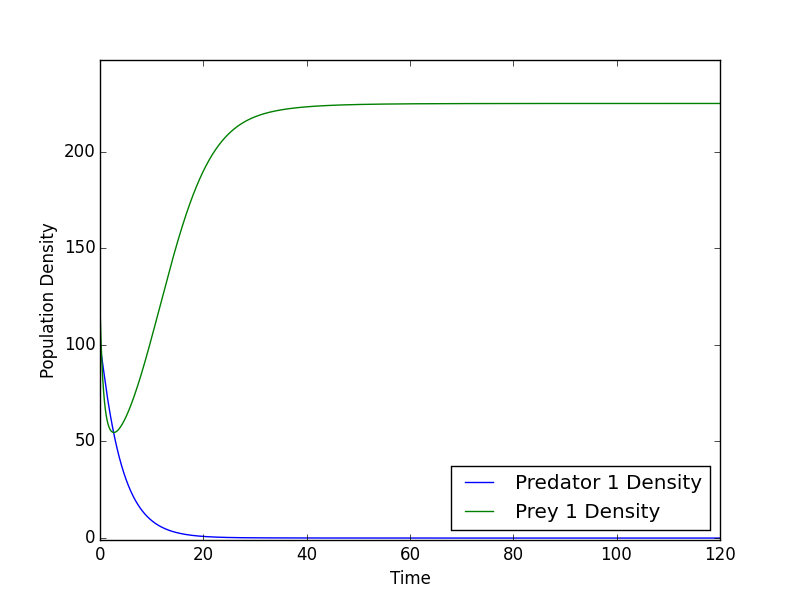
\includegraphics[scale=0.3175]{figures/1x1/densities_exclusion.png}
   	\hfill
   	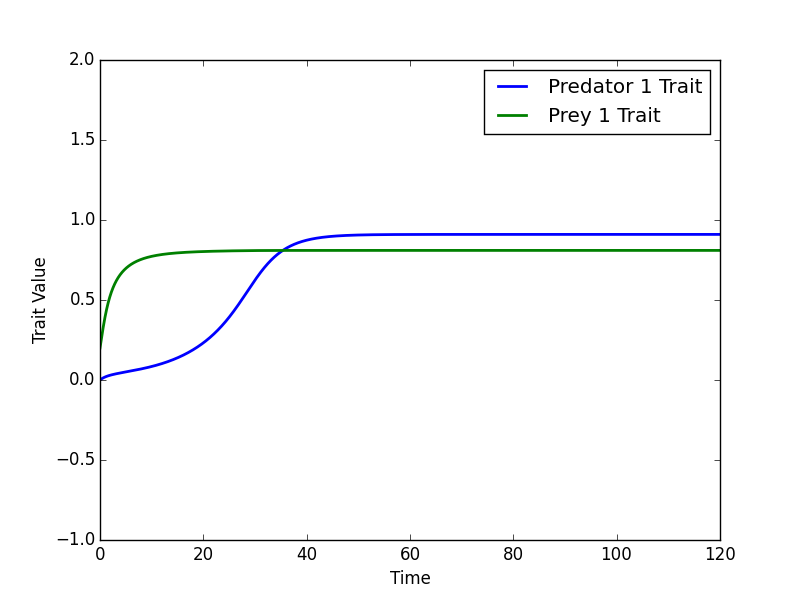
\includegraphics[scale=0.3175]{figures/1x1/traits_exclusion.png}
	}
\end{frame}
\begin{frame}
	\frametitle{Figures - $1\times1$}
	{\bf Stable Coexistence}
	\Wider[6em]{
	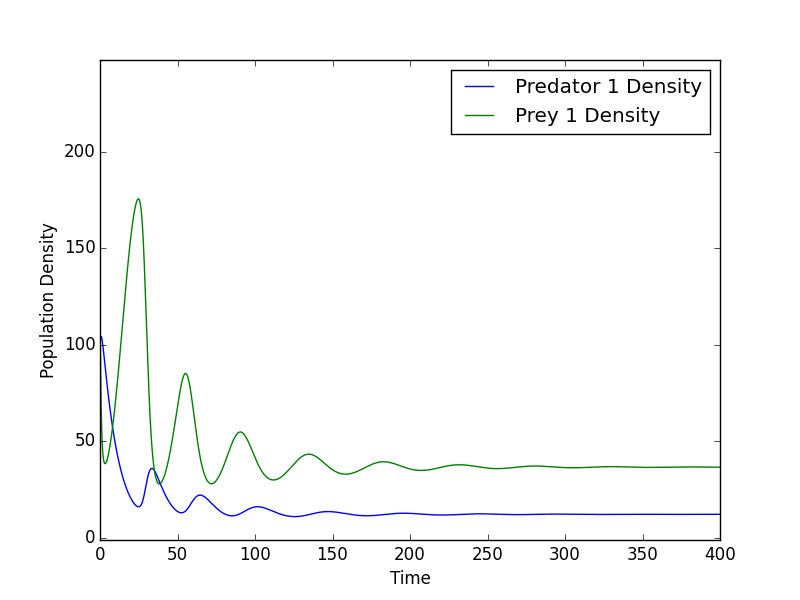
\includegraphics[scale=0.3175]{figures/1x1/densities_stable_coexistence.png}
   	\hfill
   	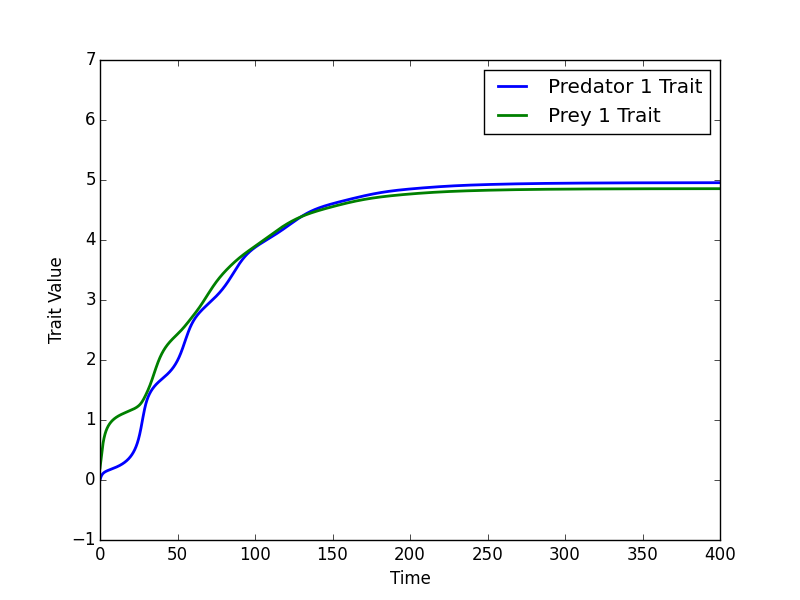
\includegraphics[scale=0.3175]{figures/1x1/traits_stable_coexistence.png}
	}
\end{frame}
\begin{frame}
	\frametitle{Figures - $1\times1$}
	{\bf Unstable Coexistence}
	\Wider[6em]{
	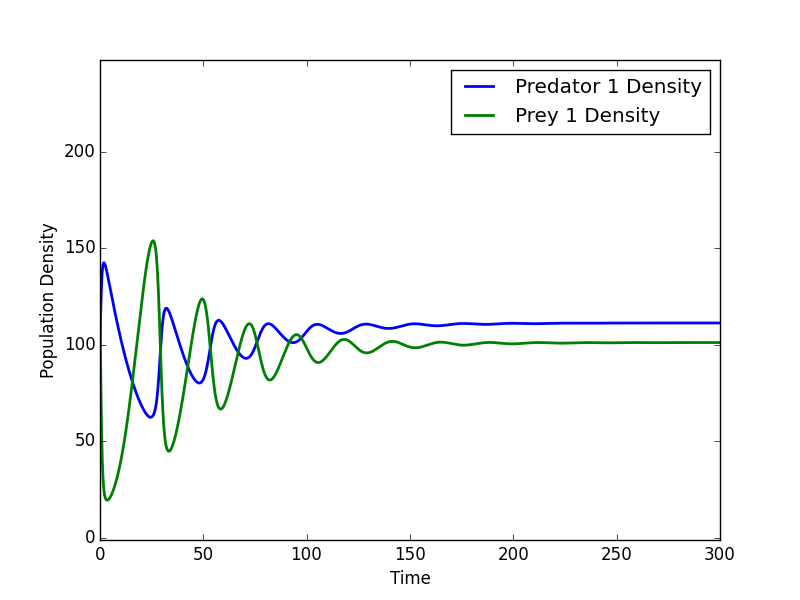
\includegraphics[scale=0.3175]{figures/1x1/densities_unstable_coexistence.png}
   	\hfill
   	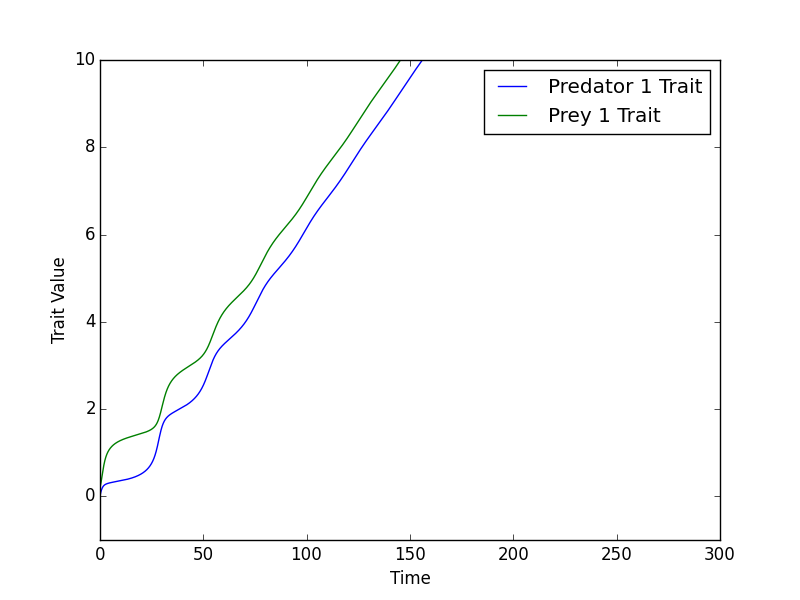
\includegraphics[scale=0.3175]{figures/1x1/traits_unstable_coexistence.png}
	}
\end{frame}

\subsection{$1 \times 2$}
\begin{frame}
	\frametitle{Equilibria - $1\times2$}
	\begin{align*}
		\begin{array}{ll}
			\dfrac{dN_1}{dt} = N_1\cdot \overline{Y}_1(\overline{m}, \overline{n}_1, M, N_1) &\ \ \ \ \ \ \dfrac{d\overline{n}_1}{dt} = \beta_{G1}^2\dfrac{\partial \overline{Y}_1}{\partial \overline{n}_1} \\[.3cm]
			\dfrac{dN_2}{dt} = N_2\cdot \overline{Y}_2(\overline{m}, \overline{n}_2, M, N_2) &\ \ \ \ \ \ \dfrac{d\overline{n}_2}{dt} = \beta_{G2}^2\dfrac{\partial \overline{Y}_2}{\partial \overline{n}_2} \\[.3cm]
			\dfrac{dM}{dt} = M\cdot \overline{W}(\overline{m}, \overline{n}_1, \overline{n}_2, N_1, N_2) & \ \ \ \ \ \ \dfrac{d\overline{m}}{dt} = \sigma_G^2\dfrac{\partial \overline{W}}{\partial \overline{m}}
		\end{array}
	\end{align*}
	\uncover<2->{{\bf Extinction}} \uncover<3->{$\boxed{\text{\it Unstable}}$}
	\begin{align*}
		\uncover<2->{(N_1^*, N_2^*, M^*, \overline{n}_1^*, \overline{n}_2^*, \overline{m}^*) = (0, 0, 0, \underline{\ \ }, \underline{\ \ }, \underline{\ \ })}
	\end{align*}
	\uncover<4->{{\bf Exclusion}} \uncover<5->{$\boxed{\text{\it Stable under certain conditions}}$}
	\begin{align*}
		\uncover<4->{(N_1^*, N_2^*, M^*, \overline{n}_1^*, \overline{n}_2^*, \overline{m}^*) &= (K_1, K_2, 0, \underline{\ \ }, \underline{\ \ }, \underline{\ \ })}
	\end{align*}
\end{frame}

\begin{frame}
	\frametitle{Equilibria - $1\times2$}
	\begin{align*}
		\begin{array}{ll}
			\dfrac{dN_1}{dt} = N_1\cdot \overline{Y}_1(\overline{m}, \overline{n}_1, M, N_1) &\ \ \ \ \ \ \dfrac{d\overline{n}_1}{dt} = \beta_{G1}^2\dfrac{\partial \overline{Y}_1}{\partial \overline{n}_1} \\[.3cm]
			\dfrac{dN_2}{dt} = N_2\cdot \overline{Y}_2(\overline{m}, \overline{n}_2, M, N_2) &\ \ \ \ \ \ \dfrac{d\overline{n}_2}{dt} = \beta_{G2}^2\dfrac{\partial \overline{Y}_2}{\partial \overline{n}_2} \\[.3cm]
			\dfrac{dM}{dt} = M\cdot \overline{W}(\overline{m}, \overline{n}_1, \overline{n}_2, N_1, N_2) & \ \ \ \ \ \ \dfrac{d\overline{m}}{dt} = \sigma_G^2\dfrac{\partial \overline{W}}{\partial \overline{m}}
		\end{array}
	\end{align*}
	\uncover<2->{{\bf Generalist Becomes Specialist}} \uncover<3->{$\boxed{\text{\it Stable under certain conditions???}}$}
	\begin{align*}
		\uncover<2->{&(N_1^*\ \ \ \ \ \ ,\ N_2^*\ ,\ M^*\ \ \ \ \ \ \ \ \ \ \ \ \ \ \ \ \ \ \ \ \ \ \ \ \ \ \ \ ,\ \overline{n}_1^*\ ,\ \overline{n}_2^*\ ,\ \overline{m}^*\ \ \ \ \ \ \ ) \\[.1cm]
		=\ &(\dfrac{d\sqrt{A_1}}{e_1 \alpha_1 \tau_1}\ ,\ K_2\ ,\ \dfrac{r_1\sqrt{A_1}}{\alpha_1\tau_1}\left(1 - \dfrac{d\sqrt{A_1}}{K_1e_1\alpha_1\tau_1}\right)\ ,\ \mu_1^*\ ,\ \mu_2^*\ ,\ \mu_1^* - \theta_1)}
	\end{align*}
	\uncover<2->{where $A_1 = \sigma^2 + \beta_1^2 + \tau_1^2$, $\mu_1^*$ is an arbitrary value, and $\mu_2^*$ is sufficiently far from $\mu_1^* - \theta_1$.}

\end{frame}

\begin{frame}
	\frametitle{Figures - $1\times2$}
	{\bf Generalist Becomes Specialist}
	\Wider[6em]{
	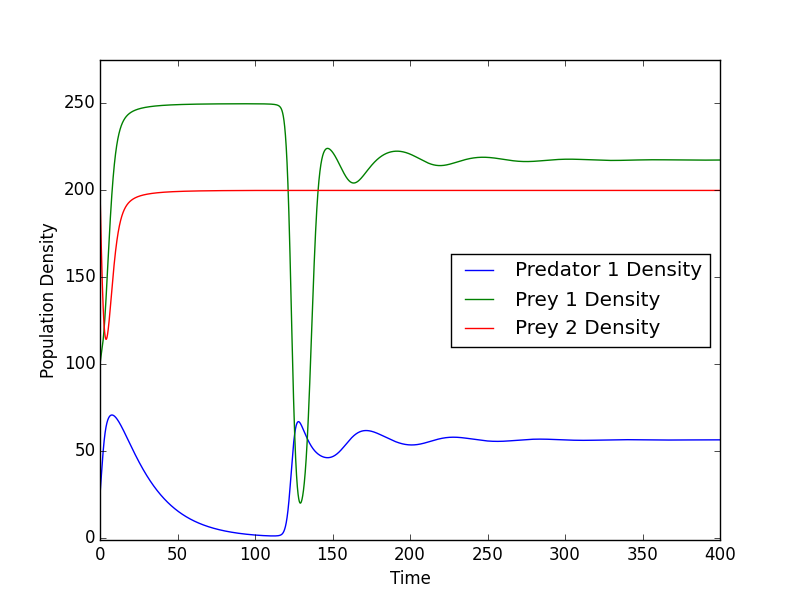
\includegraphics[scale=0.3175]{figures/1x2/densities_generalist_to_specialist.png}
   	\hfill
   	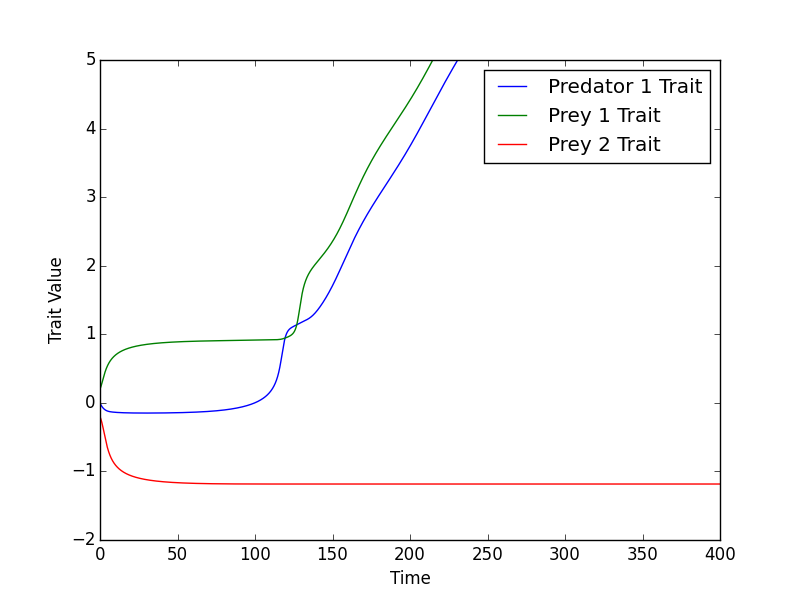
\includegraphics[scale=0.3175]{figures/1x2/traits_generalist_to_specialist.png}
	}
\end{frame}
\begin{frame}
	\frametitle{Figures - $1\times2$}
	{\bf Unstable Coexistence}
	\Wider[6em]{
	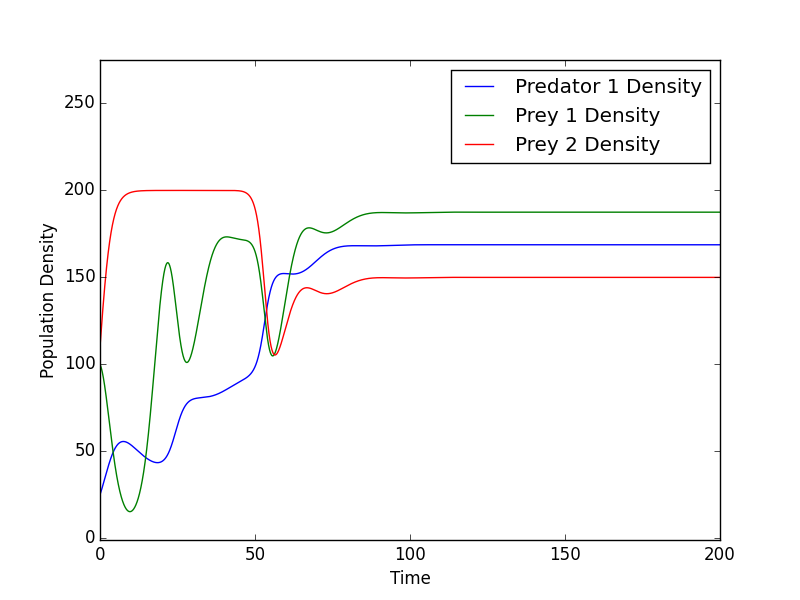
\includegraphics[scale=0.3175]{figures/1x2/densities_unstable_coexistence.png}
   	\hfill
   	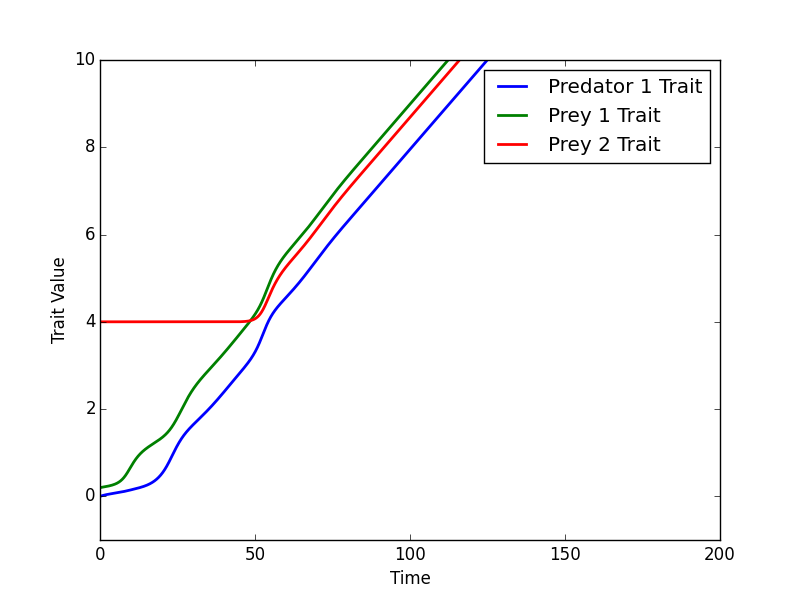
\includegraphics[scale=0.3175]{figures/1x2/traits_unstable_coexistence.png}
	}
\end{frame}

\section{Possible Expansions}
\begin{frame}
	\begin{itemize}
		\item Two Predators competing for One Prey
		\item One Specialist Predator Competing with One Generalist Predator for Two Prey Species
		\item Two Specialist Predators Competing with One Generalist Predator for Two Prey Species
		\item Further Analysis of the General $u \times v$ Model
		\item Intra-Guild Predation
		\item Adding Evolutionary Cost to Prey
		\item Adding Evolutionary Cost to Predator
	\end{itemize}
\end{frame}

\section{Thank You}
\begin{frame}
	\frametitle{Thank You!}
	\begin{itemize}
		\item Pacific Coast Undergraduate Math Conference
		\item Dr. Alissa Crans, Dr. Karrolyne Fogel, Dr. Kendra Killpatrick, Dr. John Rock, and all other PCUMC Organizers
		\item National Science Foundation
		\item Mathematical Association of America and all other PCUMC sponsors
		\item Cal Lutheran University and all other PCUMC university supporters
		\item Dr. Helena Noronha
		\item Pacific Math Alliance PUMP Undergraduate Research Groups
		\item California State University, Northridge
		\item Dr. Jing Li and Dr. Casey terHorst
	\end{itemize}
\end{frame}
\begin{frame}
	\frametitle{}
	\begin{center}
		{\Huge Questions?}
	\end{center}
\end{frame}

\section{Thanks}





\end{document}